\documentclass{standalone}
\usepackage{tikz}

\begin{document}

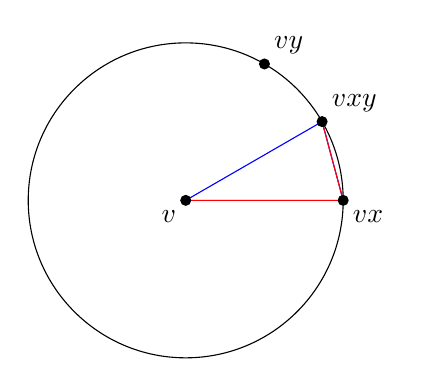
\begin{tikzpicture}[scale=2]
    % Draw the circle
    \draw (0,0) circle (1);
    
    % Define points on the circle
    \coordinate (v) at (0,0);
    \coordinate (vx) at (1,0);
    \coordinate (vy) at ({cos(60)},{sin(60)});
    \coordinate (vxy) at ({cos(30)},{sin(30)});
    
    % Draw the triangle
    \draw[blue] (v) -- (vx) -- (vxy) -- cycle;
    
    % Draw the red line
    \draw[red] (v) -- (vx);
    \draw[red] (vx) -- (vxy);
    
    % Label the points
    \fill (v) circle (1pt) node[below left] {$v$};
    \fill (vx) circle (1pt) node[below right] {$vx$};
    \fill (vy) circle (1pt) node[above right] {$vy$};
    \fill (vxy) circle (1pt) node[above right] {$vxy$};
\end{tikzpicture}

\end{document}